%%%%%%%%%%%%%%%%%%%%%%% file template.tex %%%%%%%%%%%%%%%%%%%%%%%%%
%
% This is a general template file for the LaTeX package SVJour3
% for Springer journals.          Springer Heidelberg 2010/09/16
%
% Copy it to a new file with a new name and use it as the basis
% for your article. Delete % signs as needed.
%
% This template includes a few options for different layouts and
% content for various journals. Please consult a previous issue of
% your journal as needed.
%
%%%%%%%%%%%%%%%%%%%%%%%%%%%%%%%%%%%%%%%%%%%%%%%%%%%%%%%%%%%%%%%%%%%
%
% First comes an example EPS file -- just ignore it and
% proceed on the \documentclass line
% your LaTeX will extract the file if required
\begin{filecontents*}{example.eps}
%!PS-Adobe-3.0 EPSF-3.0
%%BoundingBox: 19 19 221 221
%%CreationDate: Mon Sep 29 1997
%%Creator: programmed by hand (JK)
%%EndComments
gsave
newpath
  20 20 moveto
  20 220 lineto
  220 220 lineto
  220 20 lineto
closepath
2 setlinewidth
gsave
  .4 setgray fill
grestore
stroke
grestore
\end{filecontents*}
%
\RequirePackage{fix-cm}
%
%\documentclass{svjour3}                     % onecolumn (standard format)
%\documentclass[smallcondensed]{svjour3}     % onecolumn (ditto)
\documentclass[smallextended]{svjour3}       % onecolumn (second format)
%\documentclass[twocolumn]{svjour3}          % twocolumn
%
\smartqed  % flush right qed marks, e.g. at end of proof
%
\usepackage{graphicx}
\usepackage{subfigure}
\usepackage{amsmath}
\usepackage[center]{caption}
\usepackage{cite}
\usepackage{xcolor}
%
% \usepackage{mathptmx}      % use Times fonts if available on your TeX system
%
% insert here the call for the packages your document requires
%\usepackage{latexsym}
% etc.
%
% please place your own definitions here and don't use \def but
% \newcommand{}{}
%
% Insert the name of "your journal" with
% \journalname{myjournal}
%
\begin{document}

\title{Four legged Guar\'a robot: from inspiration to implementation%\thanks{Grants or other notes
%about the article that should go on the front page should be
%placed here. General acknowledgments should be placed at the end of the article.}
}
%\subtitle{Do you have a subtitle?\\ If so, write it here}

%\titlerunning{Short form of title}        % if too long for running head

\author{Ant\^onio Bento F \\ %\and
        Rafhael M Andrade \\	%\and 
        Cristiane P Tonetto	%etc.
}

%\authorrunning{Short form of author list} % if too long for running head

\institute{           
         F. Author \at
            Ant\^onio Bento Filho\\
            Tel.: +55-27-40092150\\
       		\email{antonio.bento@ufes.com}           %  \\
\and		S. Author \at
			Rafhael Milanezi de Andrade\\
			Tel.: +55-27-40092154\\
			\email{rafhael.andrade@ufes.com}           %  \\
			%             \emph{Present address:} of F. Author  %  if needed
			\and 
			T. author \at
			Cristiane Pescador Tonetto\\
			Tel.: +55-27-40092140\\
			\email{cristiane.tonetto@ufes.com}           %  \\
}

\date{Received: date / Accepted: date}
% The correct dates will be entered by the editor


\maketitle

\begin{abstract}
%Insert your abstract here. Include keywords, PACS and mathematical
%subject classification numbers as needed.
We present the sixteen-degree-of-freedom four-legged robot Guar\'a. Biologically inspired navigation and balance strategies were implemented through an incremental algorithm for running straight and curved paths which allows the robot to be driven on the fly, keeping it balanced. We used walking pattern matrices in statically stable walking for leg's movements coupling to run the real robot. An integrated environment was provided for walking simulation, robot's parameters adjustment and diagnosis of operation. Straight and curved path  walking results are presented, focusing on leg's kinematics and robot's stability concerns. The results show a good general performance, which encourages robot's use as a four legged research platform for indoor and outdoor applications with dynamically stable walking.
\keywords{legged robot\and mobile robot \and quadruped \and biological inspiration}
% \PACS{PACS code1 \and PACS code2 \and more}
% \subclass{MSC code1 \and MSC code2 \and more}
\end{abstract} 

\section{Introduction}
\label{intro}
The coordination of the great number of degrees of freedom that must be actuated with relative precision to a simple movement of the robot starting from point A to point B is one of the main difficulties. The challenge is to map, in very small time intervals, the simple task of moving from A to B at joints angles and trajectories, which typically must meet various constraints while still avoiding fixed and mobile obstacles \cite{berkemeier1998}. Legged robots have been design for different applications in the last few decades \cite{bares1999, kar2003, raibert2008, ponticelli2008, goncalves2015}. Comparing to wheeled and tracked locomotion, legged robots present superior mobility in natural terrains, and it can be used for both flat and rough terrains \cite{kumar2013}. On smooth floor, legged robots can walk \cite{chen2016,kar2003}; run \cite{heim2016,raibert2008} and jump \cite{kumar2013}; on the other hand in rough or slop terrains they can change their postures to obtain appropriate stability \cite{rebula2007,chen2018}.These robots can also overcome obstacles during different types of activities such as, steps \cite{nowicki2017}, rocks \cite{kimura2007}, among others. 
The robot leg is a key point of its design. Depending on the task, type of terrain and obstacle, legged robots need different mechanical characteristics of leg. Kumar and Pathak \cite{kumar2013} study a four legged jumping robot with compliant legs. The legs consist of two actuated joints, one in the rip one in the knee of the robot, and a spring and damper in parallel in the robots’ shank. Chen et al. \cite{chen2016} presents a six-legged robot, whose legs are composed by three actuator joints, two in the hip and one in the knee. The robot legs are similar to those of quadruped animals, but the knees of the first pair of legs is facing forward, and the other two pairs are facing back. Focchi et al. \cite{focchi2017} presents a four legged robot for walking in high-slope. The robot legs are similar to those presented in Chen et al. \cite{chen2016}, with two actuated joint in the hip and one in the knee. Hoffmann and Simanek \cite{hoffmann2017} presented a compliant legged with just one actuated joint in the robot hip and a passive rotation knee joint facing backward with springs attached. Rodrigues et al. \cite{rodrigues2011} presented a mechanical scheme for a leg to be included in legged vehicles that simplifies the control actuations along.
Robot navigation is another challenge in its design. It must include posture control \cite{chen2018} and stability control \cite{rebula2007} for different kind of terrain. 
This study presents the four-legged Guar\'a robot. Different of previous studies, Guar\'a's leg presents four actuated joints, two in the hip, one in the knee, and one in the foot to producing movements similar to those in quadruped animals. This leg configuration allows better possibility of impedance variation and greater flexibility of movement. The Toe-off is a movement that is only implemented in more sophisticated humanoid robots \cite{griffin2017}. With the proposed ankle joint it is possible to perform plantar flexion and dorsiflexion movements, allowing to study the toe-off and its influence on the kinematics of the robot. The Guar\'a's knees are facing forward, this configuration allows to reduce the knee joint angles with compensatory hip movements, avoiding to reach the kinematic limit of the knee joint. With four equal legs the robot's kinematics become simpler, which facilitates control and reduces the overall operating cost of the robot’s navigation system. The navigational strategy adopted in this first approach was based on the pattern of walking of most quadruped animals in flat terrains \cite{berkemeier1998} and implemented through walking matrices for indoor navigation. In addition, the robot's structure allows it to be transformed into a stable dynamic robot if the actuators are modified. Several walking control strategies can be implemented: Meta stable locomotion \cite{byl2008}, robot cooperation \cite{rocha2011}, among others, which makes the Guar\'a robot an excellent platform for research and teaching.\\
This paper is organized as follows. The legged walking robot Guar\'a design is presented in section 2. Section 3 presents the forward and inverse kinematics of the robot. In section 4 is presented the walking pattern strategy, considering a straight forward, curves and obstacles overcome trajectories. The experimental results are shown in Section 5 and Section 6 presents the final remarks of this work.

\section{Robot design}
%\subsection{Design insights for the robot}
Figure \ref{fig:fotoLoboGuara} shows a photo of guar\'a wolf, a species of canid endemic to South America and unique member of the genus Chrysocyon. This work presents the Guar\'a robot with statically stable features, walking straight and curved paths, detecting obstacles through switches on the feet, and overcoming them, following the switch collision patterns, according to its kinematic limits, or to avoid then. The robot's and leg's design have been conceived for dynamically stable walking, to come in future work.  
\begin{figure}[htb!]
	\begin{center}
	\subfigure[Guar\'a wolf with the robot's inspired structure.]{
	\includegraphics[width=0.5\textwidth]{./Figuras/guara.png}%\include
	\label{fig:fotoLoboGuara}       
	}   
	\subfigure[Guar\'a robot schematics.]{
	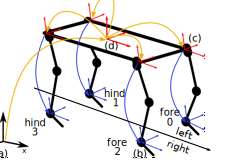
\includegraphics[width=0.45\textwidth]{./Figuras/guara_esquematico.png}
	\label{fig:guara_esquematico}}
	\caption{Biologically inspired robot Guar\'a.}
	\end{center}
\end{figure}

\subsection{Leg design} 
Humans and animals locomotion are complex phenomena in which a great number of individual motions occurs simultaneously in the three planes of space and it has been widely adopted the concept that it is the center of mass (CoM) translation of through space along a pathway requiring the least expenditure of energy. It has been  observed in humans \cite{inman_major_1953,mcmahon_muscles_1984,mcmahon_mechanics_1984,rose_human_1994} that a normal step kinematics describes six movements, used to increase the step length and flatten the inverted pendulum path of the hip, by increasing and decreasing leg's effective length, to smooth the transition between phases of leg support and transferring the body's weight on the supporting leg during foot transition. \\
The mechanical approach for our quadruped's locomotion, uses  a similar geometry and DOF layout of human leg for a four-legged machine, which would be energetically efficient and, with a suitable mechatronic design, could allow geometries like that of quadruped animal's fore and hind limbs when pushing their body. It's proposed a robotic leg having hip roll and pitch DOFs,which allows hip flexion/extension and abduction/adduction, knee pitch DOF, which allows knee flexion/extension, and and ankle  pitch DOF, which allows ankle dorsiflexion/plantarflexion. Combining them through an adequate kinematics will provide the same basic leg's movements former described.\\
Future work will attempt to improve leg's fourth DOF and foot as metatarsal and metacarpal bones (Fig. \ref{fig:guara_esquematico}, first leg segment upper to the feet), present in speedy running animals like lions, wolves, dogs and others.\\  
Being the leg implemented with a flat foot and not performing toe-off and hell-strike movements, the robot must lower itself before start walking to make room for the leg's length increase and decrease needed for moving the robot. In fig. \ref{fig:leg-takeOff} it's shown rear right leg ready to take-off then in Fig. \ref{fig:legFlight} it's flying and then in Fig. \ref{fig:legLanding} it's landing to start new support/thrust cycle. It can be notice the other legs supporting/trusting the robot having their knees a bit bent. In fig. \ref{fig:GuaraInclinado} it's shown lateral movement for legs abduction/adduction movements. They are used to move robot's CoM into supporting feet triangle shown in Fig. \ref{fig:waveGaitSupportPolygons}.\\
  Also in this research, we kept front and rear legs with knees angled forward, although the front and back paws of the animals move with their knees at inverted angles, to simplify the movements in statically stable walking. The focus is to make the robot develop straight and curved walking paths at low velocity using the last leg link resembling the humans	 feet. Future works will focus in performing toe-off and hell-strike movements with the actual legs configuration, to use leg's link four as in guar\'a wolf hind leg legs , and to improve leg's kinematics limits and power train for the robot to jump, trot and gallop, with dynamically stable balancing.
\begin{figure}[t]
	\centering
	\subfigure[Leg take off.]{\includegraphics[scale=0.475]{./Figuras/leg3TakeOff.png}
		\label{fig:leg-takeOff}
	}
	\subfigure[Leg flight.]{\includegraphics[scale=0.475]{./Figuras/leg3Flight.png}
		\label{fig:legFlight}
	}
	\subfigure[Leg landing.]{\includegraphics[scale=0.475]{./Figuras/leg3Landed.png}
		\label{fig:legLanding}
	}
	\subfigure[Lateral movements to improve robot' balance.]{\includegraphics[scale=0.2]{./Figuras/GuaraInclinado.png}
		\label{fig:GuaraInclinado}
	}
	\caption{Typical leg take-off, flight and landing to a new stroke position.}
\end{figure}
\subsection{Schematic of the Robot}
Figure \ref{fig:guara_esquematico} shows robot's global reference frame(RF)(a), CoM RF (d), leg's RF (c), foot RF (b) and feet's positions and numbering. The leg design resembles a four revolute joints manipulator which RF origin is on hip joint labeled (c). Each leg's RF origin has a position vector from CoM and leg's joint RF are in accordance to Denavit-Hartenberg convention \cite{spong_robot_2006}. 
%\subsection{Robot dimensions and kinematic limits} 
Figure \ref{fig:guaravistas} presents robot's side and back views with main dimensions; angular kinematic limits are shown in Fig. \ref{fig:legKinematicLimits} as for the leg going through hip and knee joint angles limits.   
\begin{figure}[t]
	\centering
	\subfigure[Robot main dimensions.]{\includegraphics[scale=0.25]{./Figuras/GuaraVistas}
		\label{fig:guaravistas}}
	\subfigure[Leg kinematic limits.]{\includegraphics[scale=0.2]{./Figuras/LegKinematicsLimits}
		\label{fig:legKinematicLimits}}
	\caption{Robot main dimensions.}
\end{figure}

\section{Kinematics}
The robot is composed by four legs with four DOF each. These legs could be understood as four robotic manipulators, with the robot's platform being used as the manipulator's base. The operational space is defined by the places that can be reached by the leg end effector.\\The leg was built with the first and second DOFs having the same origin, with zero link size in the first link. The DOFs are defined as roll and pitch for joint 0, and roll for joint 1, 2 and 3. The Table \ref{t:parameters} present platform and robot's legs dimensions.
\begin{table}[h]
	\centering
	\begin{tabular}{|c|r|}
		\hline
		Length between legs & 415 [mm] \\ \hline
		Width between legs & 305 [mm] \\ \hline
		Legs upper link & 150 [mm] \\ \hline
		Legs lower link & 150 [mm] \\ \hline
		Ankle height & 50 [mm] \\ \hline
		Total weight & 16 [kgf] \\ \hline
	\end{tabular}	
	\caption{Robot dimensions.}% 
	\label{t:parameters}
\end{table}
\subsection{Direct Kinematics}\label{subsectionFK}
As for the direct kinematics of the quadruped robot, the link configuration of each leg is computed as independent from the others, by using Denavit-Hartenberg (DH) parameters \cite{bento_filho_modeling_2007}. The DH parameters can be seen on Table \ref{tab:01}. The parameters are the same for all legs, assuming a local origin on their base.  There are transformations between the platform's coordinate system (located on its CoM) and the origins of each leg. Similarly, there os a transformation between the fixed reference frame (external to the robot) and the platform's coordinate system. In the Figure \ref{fig:PernaComReferenciaisDH} the position on these relevant coordinate system are depicted. 
\begin{table}[h]
	\caption{DH parameters \cite{spong_robot_2006} for the robot's legs.} %\ref{fig:PernaComReferenciaisDH}.}% 
	\begin{center}
		\begin{tabular}{crrrr}
			\label{tab:01}
			$link$ 	& $a_i$		& $d_i$		& $\alpha_i$ 		& $\theta_i$ \\ \hline
			1    	& 0			& $d_1$ 	& $\frac{\pi}{2}$ 	& $\theta_1$ \\
			2    	& $a_2$ 	& 0 		& 0 				& $\theta_2$ \\
			3    	& $a_3$ 	& 0 		& 0 				& $\theta_3$ \\
			4    	& $a_4$ 	& 0 		& 0 				& $\theta_4$ \\ \hline
		\end{tabular}		
	\end{center}
\end{table}
\begin{figure}[h]
	\centering
	\subfigure[Reference frames for the platform and legs.]{\includegraphics[scale=0.5]{./Figuras/RefGuara_V1.png}
%	\caption{Referenceframes for the platform and legs.}
	\label{fig:PernaComReferenciaisDH}
	}\\
%\end{figure}
%\begin{figure}[!h]
%	\centering
	\subfigure[DH parameters for one of the robot's  legs.]{\includegraphics[width=0.25\linewidth]{./Figuras/PernaDH}
%	\caption{DH parameters for one of the robot's legs.}
	\label{fig:Perna_DH}
	}
\caption{Robot's reference frames.}
\end{figure}
Figure \ref{fig:Perna_DH} shows the DH parameters for one of the robot's legs. This parameters are replicated for each leg. \\
For each leg the joints positions are defined by the homogeneous transformations, by using DH parameters. The matrices are presented on Equation \ref{eq:01}, using compact representation, in which $s_i=\sin(\theta_i)$ and $c_i=\cos(\theta_i)$. It can be notice that $d_1$ is the distance between the origin of joint 1 and 2 and is assumed as $d_1$ = 0, as per construction.
\begin{equation} 
\label{eq:01}
\mathbf{A_1^0} = \left[
\begin{array}{cccc}
c_1 & 0 & s_1  & 0 \\
s_1 & 0 & -c_1 & 0 \\
0  & 1 &  0   & d_1 \\
0  & 0 &  0   & 1
\end{array} \right] (a) \hspace{0.1\textwidth} \nonumber
%\end{equation}
%\begin{equation}
%\label{eq:02}
\mathbf{A_2^1} = \left[
\begin{array}{cccc}
c_2 & -s_2 & 0 & a_2c_2 \\
s_2 & c_2  & 0 & a_2s_2 \\
0  &  0   & 1 &   0    \\
0  &  0   & 0 &   1
\end{array} \right] (b) \hspace{0.1\textwidth} \nonumber
\end{equation}
\begin{equation}
%\label{eq:03}
\mathbf{A_3^2} = \left[
\begin{array}{cccc}
c_3 & -s_3 & 0 & a_3c_3 \\
s_3 & c_3  & 0 & a_3s_3 \\ 
0  &  0   & 1 &   0    \\ 
0  &  0   & 0 &   1       
\end{array} \right]  (c) \hspace{0.1\textwidth} \nonumber          
%\end{equation}      
%\begin{equation}
%\label{eq:04}
\mathbf{A_4^3} = \left[
\begin{array}{cccc}
c_4 & -s_4 & 0 & a_3c_4 \\
s_4 & c_4  & 0 & a_4s_4 \\
0  &  0   & 1 &   0    \\
0  &  0   & 0 &   1
\end{array} \right] (d) \hspace{0.1\textwidth} \nonumber
\end{equation}
\begin{equation}
\label{eq:05}
%\mathbf{X} = \left[
{A_i}^{i-1}\,=\left[
\begin{array}{cccc}
c_{\theta_i} & -s_{\theta_i}c_{\alpha_i}  & s_{\theta_i}s_{\alpha_i}  & a_ic_{\theta_i}\\
s_{\theta_i} & c_{\theta_i}c_{\alpha_i}  & -c_{\theta_i}s_{\alpha_i}  & a_is_{\theta_i}\\
0 & s_{\alpha_i} &c_{\alpha_i}  & d_i\\
0 & 0 & 0 & 1 
\end{array} \right](e)
\end{equation}	
%\paragraph{Turning}Figure \ref{fig:diagramafazendocurva} shows robot's body positions and leg's stroke when turning. The robot performs incremental arcs $θ$ with radius $R_{CoM}$, external and internal curvature radius $R_e$ and $R_i$, $\lambda_e$ and $\lambda_i$ internal and external leg's stroke and W and L robot's length and width, respectively. 
%\begin{figure}
%	\centering
%	\includegraphics[scale=0.5]{./Figuras/DiagramaFazendoCurva_}
%	\caption{Turning kinematics.}
%	\label{fig:diagramafazendocurva}
%\end{figure}
\subsection{Inverse Kinematics}
Typically for a 6 DOF's manipulator it's possible to decouple the three link from the wrist and then use geometric methods to get robot's first three DOF's and get the wrist inverse kinematics analytically \cite{spong_robot_2006}. For a four DOF leg it as in \cite{bonitz_mars_1997}. Regarding to Fig. (\ref{fig:PernaComReferenciaisDH}) , applying cosine law between links one and two, it comes:
\begin{eqnarray}
	\cos(\theta_3)=\frac{x_3^2+y_3^2+z_3^2-(a_2^2+a_3^2)}{2a_2a_3}:=D\nonumber \\
	\theta_3= atan2\,\left(\frac{\sqrt{1-D^2}}{D}\right) \label{eq:theta3}	
\end{eqnarray}
where $x_3^2, y_3^2$ and $z_3^2$ are joint three origin $O_3$ space coordinates and $a_2$ and $a_3$ are links two and three lengths respectively, and \textit{atan2} compute the arc tangent function taking into account the sign of both arguments in order to determine the quadrant. Similarly, for joint 3 we can get:
\begin{eqnarray}
\theta_2=atan2\left(\frac{z_3}{\sqrt{x_3^2+z_3^2}}\right)-atan2\left(\frac{a_3\sin 		\theta_3}{a_2+a_3 \cos \theta_3}\right)	 \label{eq:theta2}
\end{eqnarray}
and
\begin{equation}
	\theta_1=atan2 \left(\frac{x_3}{y_3}\right)  \label{eq:theta1}
\end{equation}
In statically stable walking, link $a_4$ can be kept in a known fixed vertical $\theta_4$ pitch angle, which allows joint 3 coordinates to be determined as follows:
\begin{equation}
\begin{bmatrix}
^0x_3\\^0y_3\\^0z_3
\end{bmatrix}^T=
\begin{bmatrix}
^0x_4-a_4\sin\theta_4\cos\theta1\\ ^0y_4-a_4 \sin \theta_4 \sin \theta_1\\^0z_4-a_4\sin \theta_4
\end{bmatrix} \label{eq:join3Coordinates}
\end{equation}
%%%%%%%%%%%%%%%%%%%%%%%
In dynamic walking, not yet implemented, joint 3 will be position controlled while joint 4 will be torque controlled to allow adjusting leg's impedance during locomotion. To avoid singularities, $\theta_3$ form Eq. (\ref{eq:theta3}) is the positive root, allowing knee-ahead (elbow-up) configurations for the leg.
\subsection{Differential Kinematics: Jacobian}
In this subsection the Jacobian matrix is described. The Jacobian allows to relate the foot velocities with the joint speeds, by establishing the Eq. \ref{eqJacobiano}. This allows the speed analysis for the joints (for example, maximum required speed) and trajectory planning by using differential kinematics.
\begin{equation}
\label{eqJacobiano}
\left[
\begin{array}{c}
 \dot{x}\\
 \dot{y}\\
 \dot{z}\\
 \omega_x\\
 \omega_y\\
 \omega_z\\
\end{array}\right]
= \mathbf{J(q)}\left[
\begin{array}{c}
 \dot{\theta_1}\\
 \dot{\theta_2}\\
 \dot{\theta_3}\\
 \dot{\theta_4}\\
\end{array}\right]
\end{equation}
The Geometric Jacobian for each leg of the robot was determinated by using the same procedure that was applied to the direct kinematics, as seen in subsection \ref{subsectionFK} \cite{Sciavicco:2000}. The Jacobian matrix is presented on the Eq. (\ref{eq:02}).
\begin{equation} 
\label{eq:02}
\mathbf{J(q)} = \left[
\begin{array}{cccc}
z_0 \times (p-p_0)\; & z_1\times (p-p_1)\; & z_2\times (p-p_2)\;  & z_3\times (p-p_3) \\
z_0 & z_1 & z_2 & z_3 \\
\end{array}\right]_{(6\times 4)}
\end{equation}
Each element of the Jacobian matrix is given by Eq. (\ref{eq:03}):
\begin{equation} 
\label{eq:03}
\begin{array}{l}
z_0=z_{0_i}\\
z_1=A_1^0 (1:3,3)\\
z_2=A_1^0 A_2^1  (1:3,3)\\
z_3=A_1^0 A_2^1 A_3^2 (1:3,3)\\
\end{array}
\end{equation}
Where $z_{0_i}$ is the axis initial direction for the leg's first joint, and $(1:3,3)$ refers to the vector composed by the first three elements of the third column of the homogeneous transformation matrix.
\begin{equation} 
\label{eq:04}
\begin{array} {l}
p_0 = O_l\\
p_1=A_1^0 (1:3,4)\\
p_2=A_1^0 A_2^1  (1:3,4)\\
p_3=A_1^0 A_2^1 A_3^2 (1:3,4)\\
p=A_1^0 A_2^1 A_3^2 A_4^3 (1:3,4)\\
\end{array}
\end{equation}
In which $O_l$ is the origin position for the leg's first joint and, $(1:3,4)$ is given by the vector composed by the first three elements of the fourth column of the homogeneous transformation matrix.\\
\paragraph{Jacobian in the force domain:} the work done by leg's reactions in operational space is equal the work done by torques in leg's joint-space. Thus, applying virtual work principle, Jacobian definition Eq. \ref{eqJacobiano} and handling the resulting expression, it comes \cite{craig_introduction_1989}:
\begin{eqnarray}
\label{eq:jacobianInForceDomain}
	F^T\cdot\delta_x=\tau^T\cdot\delta_{\theta}\rightarrow
	F^TJ\delta_{\theta}=\tau^T\cdot\delta_{\theta}\rightarrow\tau=J^TF
\end{eqnarray}
where $F$  is the generalized force vector on the foot, $J$ is leg Jacobian in leg's RF and $\tau$ is the leg joints torque vector. Equation \ref{eq:jacobianInForceDomain} allows leg's joint torques and ground reaction control to be implemented through joints driven by DC gear-motor current which is proportional to the DC motor torque output. 
%\subsection{Leg dynamical model}
\section{Wave gaits}%Gait modeling}%Walking}
\label{sec:walking}
%The biomechanics is the study of the mechanical laws relating to the movement or structure of living organisms. 
The mechanical study of human beings, of animals and ground insects, their walking and jumping capabilities, has inspired the mathematical modeling of their locomotion. After the modeling, it is possible to build kinematic and dynamic models for the description of their behavior, and the constructions of machines that could mimic their abilities\cite{song_machines_1989,schmiedeler_mechanics_1999,migliore_biologically_2005,semini_design_2011,michele_focchi_online_2017}.
It's observed that animals and insects use wave gaits, which have been widely implemented in walking machines, because they have the optimum stability if leg pitch P, which is the distance between the centers of two adjacent legs strokes, is greater than leg stroke R, which is the travel distance of a foot on the ground with respect to the body. Also, the quadrupedal generalized wave gaits have the best stability among all periodic gaits \cite{ZHANG19931}.
%\paragraph{Guar\'a wave gait:} 
\subsection{Gait modeling}
\label{subs:gaitModeling}
Guar\'a uses a regular symmetrical full cycle periodic natural sequence wave gait as in \cite{song_machines_1989}, which is shown in Fig. \ref{fig:WaveGaitGraph}. In this implementation, the gait cycle is divided in 32 slices, being 27 for leg's support-stroke and 5 for the leg-flight to a new position. Four legs are on support during 3 slices when the robot starts walking, and after each leg flying lands, to perform body's lateral movement. The wave gait load factor is $\beta=0.875$ and leg's phase angles are $\phi_0=0,\,\phi_1=0.75,\,\phi_2=0.5\,\text{and}\,\phi_3=0.25$ \cite{bento_filho_modeling_2007}. Figure \ref{fig:gaitLateralMovement} shows the synchronized body lateral movement used to better balance the robot by moving its CoM towards the support polygon, which improves robot's safety margin. Figure \ref{fig:waveGaitSupportPolygons} (a) to (f) shows robot body and support polygon to perform a complete gait cycle.
\begin{figure}[h]
	\centering
	\subfigure[Regular symmetrical full cycle periodic wave gait.]{\includegraphics[scale=0.43]{./Figuras/GaitGraph_v1}
		\label{fig:WaveGaitGraph}}	
	\subfigure[Synchronized robot's body lateral movement.]{\includegraphics[scale=0.47]{./Figuras/GaitCycleLateralMovement_v1}
		\label{fig:gaitLateralMovement}
	}
	\subfigure[Full gait cycle support polygons.]{\includegraphics[width=1\linewidth]{./Figuras/WaveGaitSteps_v1}
	\label{fig:waveGaitSupportPolygons}
	}
	\caption{Wave gait characteristics.}
      % Give a unique label
\end{figure}
\subsection{Turning gait}
\label{subs:turningGait}
Figure \ref{fig:diagramafazendocurva} shows robot's body positions and leg's stroke when turning. The robot performs incremental arcs $\theta$ with radius $R_{CoM}$; external $R_e$ and internal $R_i$ curvature radius define $\lambda_e$ and $\lambda_i$, respectively internal and external leg's stroke, being W and L robot's length and width, respectively. 
The incremental turning step width is set for the robot CoM path. To perform a $R_{CoM}$ right turn, as shown in Figure \ref{fig:diagramafazendocurva}, the inner and outer leg's stroke becomes $\lambda_i=R_i\theta\cos(\theta)$ and $\lambda_e=R_e\theta\cos(\theta)$.\\The four-legged turning, besides of being a position vector rotation problem, was geometrically modeled in a very simple way, by knowing that, although there are four legs RF, they are rigidly connected to each other by the robot's body with constrained movements. This allows yaw kinematic modeling save computational effort to update and rotate the position vectors. It becomes even lighter from hardware view because the angular increments for the turning are added to foot coordinates in feet operating space before being mapped to joint space.
\begin{figure}
	\centering
	\includegraphics[scale=0.5]{./Figuras/DiagramaFazendoCurva_}
	\caption{Turning kinematics.}
	\label{fig:diagramafazendocurva}
\end{figure}
\section{Results and Discussion}
It was built a four legged sixteen DOF robot shown on Figure \ref{fig:fotoRoboGuara} which legs shown in Fig. \ref{fig:PernaComponentes} are bolted to an aluminum frame. Over the frame comes robot's control, power and communication hardware. The legs have four degrees of freedom each, and works as manipulators  attached to robot's platform which operating space is defined by the feet pathways. For the purposes of kinematic analysis, the platform and legs are supposed to be a system of rigid bodies, and the leg's footholds always form a plane which will be parallel to the bearing surface if neither foothold is on an elevation or depression on the floor. \\
Leg as built mechanics can be seen on Fig. \ref{fig:PernaComponentes}. Leg roll DOF joint motor is on the external case fixed to robot's frame. Hip, knee and ankle pitch DOF's joint DC gear-motors are on leg support case, lowering legs inertia by keeping gear-motors inertias only moved by hip-roll DOF gear-motor. Except leg roll DOF, all DOFs are driven by synchronizing belts. 
\begin{figure}
	\centering
	\subfigure[Guar\'a as built photo.]{\includegraphics[scale=0.225]{./Figuras/FotoGuara.png}
	\label{fig:fotoRoboGuara} 
	}
	\subfigure[Leg mechanics.]{\includegraphics[scale=0.28]{./Figuras/PernaComponentes.png}
		\label{fig:PernaComponentes}
	}
	\caption{Robot as built.}
\end{figure} 
\\Foot pathway is shown in Fig. \ref{fig:xz}. The ideal path for foot flight to a new stroke position would be a cycloid which has an instantaneous point of zero velocity when the foot starts flying and lands. However, as the foot pathway is position controlled, due to small disturbances in robot's movements, the foot starts taking-off  pushing the feet ahead while it's still in support or, when foot is still moving ahead flying to a new stroke position, it lands. Using a polygonal path with foot take-off and landing velocities synchronized with the robot, could improve robot's overall balance, even though some small deviations occurred when foot lands. In future work, force and impedance controllers will be implemented to deal with these disturbances, improving robot's balance.
\begin{figure}[htb!]
	\centering
	\includegraphics[width=1\linewidth]{./Figuras/XZ}
	\caption{Full step foot Z coordinates.}
	\label{fig:xz}
\end{figure}
\\Figure \ref{fig:xyz} shows foot references sent to and received from the robot. The individual feet's planned pathways are generated according to the walking scheme depicted in subsections \ref{subs:gaitModeling} and \ref{subs:turningGait}. The controllers on board the robot then track with good accuracy as shown, allowing the robot to walk. Dotted lines are references sent and continuous lines are executed by robot controllers. 
\begin{figure}[htb!]
	\centering
	\includegraphics[width=1\linewidth]{./Figuras/xyz}
	\caption{Full step foot 3 X, Y and Z coordinates.}
	\label{fig:xyz}
\end{figure}
\begin{figure}[htb!]
	\centering
	\includegraphics[width=1\linewidth]{./Figuras/x}
	\caption{Foot 3 X coordinates.}
	\label{fig:gaitFlightAndThrustPathway}
\end{figure}
\begin{figure}[htb!]
	\includegraphics[width=1\linewidth]{./Figuras/y}
	\caption{Robot's body lateral movement.} 
	\label{fig:y}
\end{figure}\\	
Figure \ref{fig:gaitFlightAndThrustPathway} shows foot being pushed from hind to fore leg's kinematic limit and back in support, thrusting the robot. First line segment is the foot going forward to a new stroke position and second is the foot thrusting, as shown in Fig. \ref{fig:xz}. Robot's side movement allows increasing static stability margin.\\ Execution of the model depict in Figures \ref{fig:WaveGaitGraph} and \ref{fig:gaitLateralMovement}Figure \ref{fig:y} shows . It can be seen in Fig. \ref{fig:y} that this side movement is done with the four legs in support phase.\\
Feet curved pathways with the robot turning right with an average radius 1.4m, 108 thrusting and 20 flying points, are shown in Figs. \ref{fig:xyLegs0&2} and \ref{fig:xyLegs0&2}.
\begin{figure}[htb!]
	\centering
	\subfigure[Feet 0 and 2, X-Y  coordinates.]{\includegraphics[width=1\linewidth]{Figuras/XY02}%{Figuras/xyLegs0&2}%xyzFeet0&2CurvedPathway.pdf}
	\label{fig:xyLegs0&2}
	}
	\hspace{0.5cm}
	\subfigure[Feet 0 and 1, X-Y  coordinates. .]{\includegraphics[width=1\linewidth]{Figuras/XY01}%{Figuras/xyLegs0&1.pdf}
		\label{fig:xyLegs0&1}
	}
	\caption{Feet curved pathways.}
\end{figure}
Figure \ref{fig:xyLegs0&2} shows front feet 0 and 2 foothold pathway referred to their leg's joint 0 RF (Fig. \ref{fig:guara_esquematico}). Continuous and dotted blue lines correspond to lateral Y pathway, pushing robot's body CoM towards inside support polygon, and are a little rotated clockwise according to the turning model proposed before (see \ref{subs:turningGait}, Fig. \ref{fig:diagramafazendocurva}).\\ 
Continuous and dotted black lines in Fig. \ref{fig:xyLegs0&2} correspond to feet 0 and 2 thrust (X) pathway. It can be seen that the dotted line has greater amplitude (from bottom to upper corner) than the continuous one, because foot 0 is turning outside the curve and has to travel a greater distance than foot 2 turning inside. \\
In Fig. \ref{fig:xyLegs0&1} it's depicted the same as in Fig. \ref{fig:xyLegs0&2}, though for left feet 0 and 1. Continuous and dashed blue lines correspond to lateral pushing of robot's body, and are a little rotated symmetrically, as both feet are left, according to the proposed turning model. Here the continuous and dashed black lines which correspond to feet 0 and 1 thrust (X) pathway, have same amplitude (from bottom to upper corner) as they have same curvatures radius and consequently have to travel equal distances. \\
Summing it up, remembering that the feet are in support, the lateral and push combined movements are imparted to robot by the modeled feet movements which are reflected to robot's body, allowing it to turn while being pushed by its legs. \\
It's worth noting that lateral displacement of robot's body, synchronized with stroke, improves its statically stability margin (SSM). The discontinuities shown in lateral Y pathway, in both figures, pushing robot's body CoM towards inside support polygon, are due to additional leg excursion necessary to lift up the foot vertically. As in this movement kinematics requires not only leg's extension or retracting, the increasing or decreasing in leg's joint 0 angle occurs for leg's flying to a new stroke position.\\
Frames taken from robot's video doing a ninety degree right turn is shown in Figs. \ref{fig:curva1} \ref{fig:curva4} and \ref{fig:curva6}. In Fig. \ref{fig:curva1}, it can be seen the right front and hind legs have joint 0 (roll) symmetrical angles; the same can be seen for left legs, in mid-turn, Fig. \ref{fig:curva4}; and ending turn is seen in Fig. \ref{fig:curva6}. Turning is done according to what was described in \ref{subs:turningGait}, validating the software simple approach to implement turning robot on-the-flight.
\begin{figure}[htb!]
	\centering
	\subfigure[Start turning.]{\includegraphics[scale=0.375]{Figuras/Curva_1}
	\label{fig:curva1}
	}
	\subfigure[Middle path turning.]{\includegraphics[scale=0.285]{Figuras/Curva_4}
	\label{fig:curva4}
	}
	\subfigure[Ending turn.]{\includegraphics[scale=0.275]{Figuras/Curva_6}
		\label{fig:curva6}
	}
	\caption{Robot's turning right with average radius 1.4 m.}
\end{figure}
\section{Conclusions and Future Work}
The Guar\'a robot, a four legged sixteen DOF mobile robot was developed and constructed, being capable of walking statically stable straight and curved paths.  \\
The leg's design with hip roll and pitch DOFs, forming a spherical joint at the point leg's attachment to robot's platform, made it possible to perform lateral displacement of the body towards its support polygon, being this one of the movements performed by the mammals during walking. It moves the CoM projection on the ground towards support polygon, which results in greater SSM for the robot during walking.\\
The hip roll DOF allows abduction-adduction of the legs, expanding feet workspace and so that feet foothold pathways curves could be any shape, inside leg's kinematic limits.\\
Straight and curved paths are generated separately and the final movement is composed by a vector sum of them operating space. With this structure stroke can be varied through pathways points number and  increments in feet workspace, which are then mapped in joint space through inverse kinematics.\\
Line segments in feet workspace for straight walking synchronizing robot's body lateral movement, allows curved walking be done with same stability criterion. With this, the radial and tangential displacement values ​​for curved and straight pathway are combined, before the mapping from feet  to leg's joint workspace. This approach doesn't need a path generation layer that would have to be executed for the robot CG in relation to the on board RF and then mapped to the leg RF through leg's to CoM position vectors. The pathway generation of of each foot is linked to the robot's body through the maneuverability scheme, but is generated in the operating space of the feet, not requiring any matrix calculations, lowering overall math process effort.
Considering this math needed to generate the four feet pathways in their workspace and mapping in leg's joint space, a walking strategy whose output can be generated at the robot's DOF activation level, allows a valuable increasing in overall robot's controller performance.\\
Results achieved encourages improvements to robot design and power train and future works with dynamically stable gaits and other stability control strategies like zero moment point (ZMP) and angular momentum \cite{byl2008,popovic_angular_2004,popovic_ground_2005}. \\
Future works will attempt to set the fourth leg's DOF resembling the metacarpals and metatarsals, bones connecting forelimb radius and hind limbs tibia to digits, present in dogs, horses, lions, wolves and others speedy animals,  which allow then to achieve high speed running, and implementing a new control framework using a quadratic program that reconciles motion tasks expressed as constraints on the joint acceleration vector \cite{koolen_design_nodate} with the limitations due to unilateral ground contact and force-limited grasping, modeled as cones friction constraints \cite{pratt_bookchapter_2016}.\\  
In future work, the leg's fourth DOF will be considered as a multi-body system\cite{tonetto_musme}, since the robot has been modeled and controlled as a cooperative robotic system, with the legs cooperating for the robot to walk.
%\begin{acknowledgements}
%If you'd like to thank anyone, place your comments here
%and remove the percent signs.
%\end{acknowledgements}
%\textcolor{red}{\section{To do}
%\begin{itemize}
%	\item OK Angulos de juntas enviados \textcolor{black}{N\~AO e recebidos} em reta e curva;
%	\item OK Coment\'arios sobre as curvas de \^angulos enviados  \textcolor{black}{N\~AO /recebidos};
%	\item NÃO \^Angulo teste isolado enviado e recebido de uma pata;
%	\item OK Comentar sobre limita\c c\~oes na ado\c c˜\~ao da cicl\'oide;
%	\item OK Descrever e comentar a trajet\'oria adotada.
%	\item \textcolor{black}{N\~AO Subir e descer degrau}
%	\begin{itemize}
%		\item \textcolor{black}{N\~AO Comentar sobre acionamentos simples;}
%		\item \textcolor{black}{N\~AO Descrever composi\c c\~ao para compor movimentos complexos a partir de padr\~oes das chaves do p\'e.}
%	\end{itemize}
%\end{itemize}
%}
% BibTeX users please use one of
%\bibliographystyle{spbasic}      % basic style, author-year citations
%\bibliographystyle{spmpsci}      % mathematics and physical sciences
%\bibliographystyle{spphys}       % APS-like style for physics
%\bibliography{}   % name your BibTeX data base

% Non-BibTeX users please use
%\begin{thebibliography}{}
%
% and use \bibitem to create references. Consult the Instructions
% for authors for reference list style.
%
%\bibitem{RefJ}
% Format for Journal Reference
%Author, Article title, Journal, Volume, page numbers (year)
% Format for books
%\bibitem{RefB}
%Author, Book title, page numbers. Publisher, place (year)
% etc
%\end{thebibliography}
\bibliographystyle{IEEEtran}
\bibliography{Guara}%/Users/antoniobentofilho/Dropbox/Latek/COBEM2017/Momentum}
\end{document}
% end of file template.tex




